\documentclass[10pt, varwidth=15cm]{standalone}

% For large-sized journals the figures should be 84 mm (for double-column text areas), 
% or 174 mm (for single-column text areas) wide and not higher than 234 mm. SAMO


\usepackage[utf8]{inputenc}
\usepackage{bm} % bold math letter
\usepackage{amsmath}
\usepackage{amsfonts}
\usepackage{stanli} % Structure Analisys tikz package
\usepackage{structmech}
\usepackage{siunitx}

% Tikz settings
\usepackage{pgfplots}
\usepackage{tikz}
\usetikzlibrary{decorations.pathreplacing,spy}
\usetikzlibrary{fit}
\usetikzlibrary{shapes.geometric}
\usetikzlibrary{shapes.arrows}
\usetikzlibrary{positioning}
\usetikzlibrary{decorations.pathreplacing,spy}
\usetikzlibrary{arrows.meta}

\pgfdeclarelayer{background}
\pgfsetlayers{background, main}
\pgfplotsset{compat=1.18}

\tikzstyle{decision} = [diamond, aspect=1.8, text centered, fill=white, draw=black, thick]
\tikzstyle{block} = [rectangle, draw=black, thick, fill=white, text centered, rounded corners, minimum height=2em]

\pgfplotsset{
    colormap={coolwarm}{
        rgb255(0cm)=(58,76,192);
        rgb255(1cm)=(64,84,199);
        rgb255(2cm)=(70,93,207);
        rgb255(3cm)=(76,102,214);
        rgb255(4cm)=(82,110,220);
        rgb255(5cm)=(90,120,227);
        rgb255(6cm)=(96,128,232);
        rgb255(7cm)=(103,136,237);
        rgb255(8cm)=(109,144,241);
        rgb255(9cm)=(117,152,246);
        rgb255(10cm)=(124,160,249);
        rgb255(11cm)=(131,166,251);
        rgb255(12cm)=(138,173,253);
        rgb255(13cm)=(145,179,254);
        rgb255(14cm)=(153,186,254);
        rgb255(15cm)=(160,191,254);
        rgb255(16cm)=(167,196,253);
        rgb255(17cm)=(174,201,252);
        rgb255(18cm)=(182,206,249);
        rgb255(19cm)=(188,209,246);
        rgb255(20cm)=(194,212,243);
        rgb255(21cm)=(200,215,239);
        rgb255(22cm)=(206,217,235);
        rgb255(23cm)=(213,219,229);
        rgb255(24cm)=(218,220,223);
        rgb255(25cm)=(223,219,217);
        rgb255(26cm)=(228,216,209);
        rgb255(27cm)=(233,212,201);
        rgb255(28cm)=(237,208,193);
        rgb255(29cm)=(240,204,185);
        rgb255(30cm)=(242,199,178);
        rgb255(31cm)=(244,194,170);
        rgb255(32cm)=(246,187,160);
        rgb255(33cm)=(247,181,152);
        rgb255(34cm)=(247,174,145);
        rgb255(35cm)=(246,167,137);
        rgb255(36cm)=(245,158,127);
        rgb255(37cm)=(243,150,120);
        rgb255(38cm)=(241,142,112);
        rgb255(39cm)=(238,134,105);
        rgb255(40cm)=(234,125,97);
        rgb255(41cm)=(230,114,89);
        rgb255(42cm)=(225,104,82);
        rgb255(43cm)=(220,94,75);
        rgb255(44cm)=(215,84,68);
        rgb255(45cm)=(207,70,61);
        rgb255(46cm)=(201,59,55);
        rgb255(47cm)=(194,45,49);
        rgb255(48cm)=(187,26,43);
        rgb255(49cm)=(179,3,38);
        },
        colormap name=coolwarm, 
        }

        \pgfplotsset{
    colormap={coolwarm_r}{
        rgb255(27cm)=(233,212,201);
        rgb255(28cm)=(237,208,193);
        rgb255(29cm)=(240,204,185);
        rgb255(30cm)=(242,199,178);
        rgb255(31cm)=(244,194,170);
        rgb255(32cm)=(246,187,160);
        rgb255(33cm)=(247,181,152);
        rgb255(34cm)=(247,174,145);
        rgb255(35cm)=(246,167,137);
        rgb255(36cm)=(245,158,127);
        rgb255(37cm)=(243,150,120);
        rgb255(38cm)=(241,142,112);
        rgb255(39cm)=(238,134,105);
        rgb255(40cm)=(234,125,97);
        rgb255(41cm)=(230,114,89);
        rgb255(42cm)=(225,104,82);
        rgb255(43cm)=(220,94,75);
        rgb255(44cm)=(215,84,68);
        rgb255(45cm)=(207,70,61);
        rgb255(46cm)=(201,59,55);
        rgb255(47cm)=(194,45,49);
        rgb255(48cm)=(187,26,43);
        rgb255(49cm)=(179,3,38);
        }
        }

\pgfplotsset{
    colormap={coolwarm_b}{
        rgb255(0cm)=(58,76,192);
        rgb255(1cm)=(64,84,199);
        rgb255(2cm)=(70,93,207);
        rgb255(3cm)=(76,102,214);
        rgb255(4cm)=(82,110,220);
        rgb255(5cm)=(90,120,227);
        rgb255(6cm)=(96,128,232);
        rgb255(7cm)=(103,136,237);
        rgb255(8cm)=(109,144,241);
        rgb255(9cm)=(117,152,246);
        rgb255(10cm)=(124,160,249);
        rgb255(11cm)=(131,166,251);
        rgb255(12cm)=(138,173,253);
        rgb255(13cm)=(145,179,254);
        rgb255(14cm)=(153,186,254);
        rgb255(15cm)=(160,191,254);
        rgb255(16cm)=(167,196,253);
        rgb255(17cm)=(174,201,252);
        rgb255(18cm)=(182,206,249);
        rgb255(19cm)=(188,209,246);
        rgb255(20cm)=(194,212,243);
        rgb255(21cm)=(200,215,239);
        rgb255(22cm)=(206,217,235);
        rgb255(23cm)=(213,219,229);
        rgb255(24cm)=(218,220,223);
        rgb255(25cm)=(223,219,217);
        }
        }
%-----------------------------
%- CUSTOM COLORS
%-----------------------------
\definecolor{accent_b_1}{RGB}{58,76,192}
\definecolor{accent_b_2}{RGB}{103,136,237}
\definecolor{accent_b_3}{RGB}{153,186,254}
\definecolor{accent_b_4}{RGB}{200,215,239}

\definecolor{accent_r_1}{RGB}{179,3,38}
\definecolor{accent_r_2}{RGB}{225,104,82}
\definecolor{accent_r_3}{RGB}{246,167,137}
\definecolor{accent_r_4}{RGB}{237,208,193}

\definecolor{axis_gray}{RGB}{120,120,120}
\definecolor{legend_gray}{RGB}{204,204,204}

%-----------------------------
%- CUSTOM NODES
%-----------------------------
\tikzstyle{point} = [circle,fill=white,draw,inner sep=0pt,minimum size=4pt]
\tikzstyle{forces} = [draw=accent_r_1,-stealth,very thick]
\tikzstyle{lab} = [align=center, fill=white,rounded corners=2pt, inner sep=1pt, font=\footnotesize]
\tikzstyle{arrow_reference} = [-{Triangle[open,length=2.8mm]}, line width=1pt]
%-----------------------------
%- MACROS
%-----------------------------
% Circled letters
\makeatletter
\usetikzlibrary{calc}
\newcommand*\circled[1]{\tikz[baseline=(char.base)]{
    \node[shape=circle, draw, inner sep=0pt, 
        minimum height={\f@size*1.4},] (char) {\vphantom{WAH1g}#1};}}
\makeatother


\newcommand{\norm}[1]{\lVert#1\rVert}
\newcommand{\vect}[1]{\bm{#1}}
\newcommand{\matr}[1]{\bm{#1}}

%-----------------------------
%- STYLE
%-----------------------------

% plot axis styles
\pgfplotsset{general2D/.style={ 
    footnotesize,
    scale only axis,
    axis x line=middle, 
    axis y line=middle, 
    xlabel={$x$}, ylabel={$y$}, 
    axis equal, 
    axis line style={-stealth,semithick},
    } 
}

\pgfplotsset{general3D/.style={ 
    scale only axis, 
    axis line style={-stealth,semithick},
    } 
}

\pgfplotsset{curves/.style={ 
        footnotesize,
        scale only axis, 
        xtick pos=left,
        ytick pos=left,
        axis x line*=bottom, % asterisk = no arrow
        axis y line*=left,
        clip=false,
        enlarge x limits={abs=0.15cm,lower},
        enlarge y limits={abs=0.15cm,lower},
        axis line style={thick, axis_gray, shorten <=0.136cm},
        every axis label/.append style ={axis_gray},
        every tick label/.append style ={axis_gray},
        every x tick/.style={color=axis_gray, thick},
        every y tick/.style={color=axis_gray, thick},
        tick align=outside,
        xlabel near ticks,
        ylabel near ticks,
        legend style={draw=none, font=\scriptsize},
        /pgf/number format/.cd,
        1000 sep={}
    } 
}

\pgfplotsset{curves_left/.style={ 
        scale only axis, 
        xtick pos=left,
        ytick pos=left,
        axis x line*=bottom, % asterisk = no arrow
        axis y line*=left,
        clip=false,
        tick label style={font=\scriptsize},
        every axis label/.append style ={axis_gray, font=\scriptsize},
        every tick label/.append style ={axis_gray},
        every x tick/.style={color=axis_gray, thick},
        every y tick/.style={color=axis_gray, thick},
        enlarge x limits={abs=0.15cm},
        enlarge y limits={abs=0.15cm},
        axis line style={axis_gray,thick, shorten <=0.136cm, shorten >= 0.136cm},
        tick align=outside,
        xlabel near ticks,
        ylabel near ticks,
        legend style={draw=none, font=\scriptsize\color{axis_gray}},
        /pgf/number format/.cd,
        1000 sep={}
    } 
}

\pgfplotsset{curves_right/.style={ 
        scale only axis, 
        xtick pos=left,
        ytick pos=right,
        axis y line*=right,
        x axis line style={draw=none},
        x tick style={draw=none},
        ytick pos=right,
        axis x line*=bottom, % asterisk = no arrow
        axis y line*=left,
        clip=false,
        tick label style={font=\scriptsize},
        every axis label/.append style ={axis_gray, font=\scriptsize},
        every tick label/.append style ={axis_gray},
        every y tick/.style={color=axis_gray, thick},
        enlarge x limits={abs=0.15cm},
        enlarge y limits={abs=0.15cm},
        axis line style={thick, shorten <=0.136cm, shorten >= 0.136cm},
        every y tick/.style={thick},
        tick align=outside,
        ylabel near ticks,
        legend style={draw=none, font=\scriptsize},
        /pgf/number format/.cd,
        1000 sep={}
    } 
}

\pgfplotsset{curves_3D/.style={ 
        footnotesize,
        scale only axis, 
        % xtick pos=left,
        % ytick pos=left,
        % ztick pos=left,
        axis x line*=bottom, % asterisk = no arrow
        axis y line*=left,
        axis z line*=left,
        clip=false,
        % enlarge x limits={abs=0.15cm,lower},
        % enlarge y limits={abs=0.15cm,lower},
        axis line style={thick, axis_gray, shorten <=0.136cm},
        every axis label/.append style ={axis_gray},
        every tick label/.append style ={axis_gray},
        every x tick/.style={color=axis_gray, thick},
        every y tick/.style={color=axis_gray, thick},
        every z tick/.style={color=axis_gray, thick},
        tick align=outside,
        % xlabel near ticks,
        % ylabel near ticks,
        legend style={draw=none, font=\scriptsize},
        /pgf/number format/.cd,
        1000 sep={},
        view={25}{40},
        colormap name=coolwarm,
    } 
}

\pgfplotsset{line_plot/.style={ 
            thick} 
}

\pgfplotsset{scatter_plot_smooth/.style={ 
    thick,
    mark size=1.5, 
    mark=*,
    mark options={solid}, 
    smooth }
}

\pgfplotsset{scatter_plot/.style={ 
    thick,
    mark size=1.5, 
    mark=*,
    mark options={solid}, 
    only marks} 
}

\pgfplotsset{scatter_plot_lin/.style={ 
    thick,
    mark size=1.5, 
    mark=*,
    mark options={solid},} 
}



\usepackage{amsmath}
% Definition of \boxed in amsmath.sty:
% \newcommand{\boxed}[1]{\fbox{\m@th$\displaystyle#1$}}

\usepackage{xcolor}
\usepackage{nicematrix}

% Syntax: \colorboxed[<color model>]{<color specification>}{<math formula>}
\newcommand*{\colorboxed}{}
\def\colorboxed#1#{%
  \colorboxedAux{#1}%
}
\newcommand*{\colorboxedAux}[3]{%
  % #1: optional argument for color model
  % #2: color specification
  % #3: formula
  \begingroup
    \colorlet{cb@saved}{.}%
    \color#1{#2}%
    \boxed{%
      \color{cb@saved}%
      #3%
    }%
  \endgroup
}

\begin{document}

\begin{tikzpicture}[square/.style={rectangle,minimum width=1.5cm,minimum
    height=1.5cm,draw=black,thick,fill=white}]
    \def\x{6.5cm}
    \def\xjump{9cm}
    \def\yjump{-3cm}

    %%%%%%%%%%%%%%%%%%%%%%%% MODULE
    
    \foreach \xa in {0,\x*2/5*1/3,\x*2/5*2/3,\x*2/5}
            \foreach \ya in {0,\x*1/10,\x*1/5}  
                    \foreach \xx in {0,\x*2/5*1/3,\x*2/5*2/3,\x*2/5}
                        \foreach \yy  in {0,\x*1/10,\x*1/5}  
                                \draw[axis_gray, thin] (\xa, \ya) -- (\xx, \yy);

    \point{a1}{0}{0};
    \point{b1}{0}{\x*1/10*2};
    \point{c1}{\x*1/5*2}{\x*1/10*2};
    \point{d1}{\x*1/5*2}{0};
    \point{e1}{\x*1/5}{0};

    \beam{2}{a1}{b1}[1][1];
    \beam{2}{b1}{c1}[1][1];
    \beam{2}{c1}{d1}[1][1];
    \beam{2}{d1}{a1}[1][1];

    %%%%%%%%%%%%%%%%%%%%%%%% BCs

    \draw[axis_gray, -stealth] (e1.south) to[out=270,in=110] (\x*1/5+\x*1/10,\yjump*0.7-0.3cm+\x*.2);
    % Draw help lines with different step sizes
    \foreach \xx in {0,\x*1/5,\x*2/5,\x*3/5,\x*4/5,\x} {
    \foreach \yy in {0,\x*.1,\x*.2} {
        \draw [help lines] (\x, \yjump*0.7+\yy) -- (0, \yjump*0.7+\yy); % Vertical lines
        \draw [help lines] (\xx, \yjump*0.7+\x*0.2) -- (\xx,\yjump*0.7+ 0); % Horizontal lines
    }
    }

    \point{a}{0}{\yjump*0.7+0};
	\point{b}{0}{\yjump*0.7+\x*.2};
	\point{c}{\x}{\yjump*0.7+\x*.2};
	\point{d}{\x}{\yjump*0.7+0};

	\beam{2}{a}{b}[1][1];
	\beam{2}{b}{c}[1][1];
	\beam{2}{c}{d}[1][1];
	\beam{2}{d}{a}[1][1];
	
	% \notation{5}{b}{c}[$F$][.05][above=4mm]
	\notation{5}{b}{c}[\scriptsize$5L$][.5][above=2mm];
	\notation{5}{c}{d}[\scriptsize$L$][.5][right=2mm][1];
	
    \begin{scope}[scale=0.5]
        \SleeveSupport{0,\yjump*0.7*2+\x*.2}[.15]{\x*.015}
        \support{2}{d}
        \hinge{1}{d}
    \end{scope}


    \draw[forces, accent_r_1] (0,\yjump*0.7-0.2cm) -- (0,\yjump*0.7-0.8cm) node[right] {\scriptsize$P/2$};
    \draw[forces, accent_r_1] (\x*1/5,\yjump*0.7-0.2cm) -- (\x*1/5,\yjump*0.7-0.8cm) node[right] {\scriptsize$P$};
    \draw[forces, accent_r_1] (\x*2/5,\yjump*0.7-0.2cm) -- (\x*2/5,\yjump*0.7-0.8cm) node[right] {\scriptsize$P$};
    \draw[forces, accent_r_1] (\x*3/5,\yjump*0.7-0.2cm) -- (\x*3/5,\yjump*0.7-0.8cm) node[right] {\scriptsize$P$};
    \draw[forces, accent_r_1] (\x*4/5,\yjump*0.7-0.2cm) -- (\x*4/5,\yjump*0.7-0.8cm) node[right] {\scriptsize$P$};


\draw[axis_gray,thick] (\x*4/5-0.1cm,\yjump*0.7+\x*1/5+0.1cm) rectangle (\x+0.1cm,\yjump*0.7+\x*1/10-0.1cm);
\draw[axis_gray] (\x+0.2cm,\yjump*0.7+\x*1/10 + \x*1/20)  to[out=0,in=180] (8,-1);

\begin{axis}[
    curves,
    width = 4cm,
    height = 3cm,
    at={(8.5cm,-1.8cm)},
    ybar,
    xtick={1,2,3},
    xmin = 0.7, xmax = 3.3,
    % xticklabels={$t=0$, $t=1$},
    xticklabels={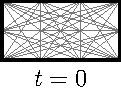
\includegraphics[width=1cm]{module_1.pdf},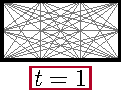
\includegraphics[width=1cm]{module_2.pdf},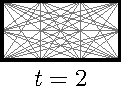
\includegraphics[width=1cm]{module_3.pdf}}, % Include images as tick labels
    ylabel={$\alpha_{t,\text{it}=0}^j$},
    ymin=0, ymax=1,
    bar width=0.4cm,
    % xmode=log,
    ytick={0,0.5,1},
    ]
    \addplot[draw=accent_b_1,fill=accent_b_2] coordinates {
      (1,0.3185) (2,0.363) (3,0.3185)
    };
  \end{axis}


% \draw [decorate,decoration={brace,amplitude=10pt},xshift=0pt,yshift=0cm]
%     (0,3.15) -- (6,3.15) node [black,midway,yshift=.6cm] {\footnotesize $N_\text{sub,x}$};
    
% \draw [decorate,decoration={brace,amplitude=10pt},xshift=0cm,yshift=0cm]
%     (6.5,3) -- (6.5,0) node [black,midway,xshift=.9cm] {\footnotesize $N_\text{sub,y}$};


%   \node[square] at (1,-2) (square1){};
%   \foreach \X [count=\Y] in {2,3,4,5,6,7,8}
%   {\node[anchor=north west,below right=2mm and 2mm of square\Y.north west,square] (square\X){};}
%   \node[fit=(square1)(square8),xshift=0.1 cm](fit1){};
%   \draw[decorate,decoration={brace}] (fit1.north east) --
%   (fit1.south east) node[midway,right,align=left,text width = 2.5cm, xshift=0.1 cm] (sub) {\small Submodules monolitic sensitivities};

%   \node[black] at (square8) {$\frac{\partial(\cdot)}{\partial \bm{a}^j}$};

% \node [black,text width=8cm, align=center] at (3.8,-5.7) {\small
% \begin{equation*}
%     \begin{split}
%         \frac{\partial(\cdot)_i}{\partial\bar{\bm{a}}_{t=0}} ={} & \colorboxed{accent_b_1}{1}\times\colorboxed{accent_r_1}{\frac{\partial(\cdot)_i}{\partial \bm{a}^0}}+\colorboxed{accent_b_1}{1}\times\colorboxed{accent_r_1}{\frac{\partial(\cdot)_i}{\partial \bm{a}^1}}+\colorboxed{accent_b_1}{1}\times\colorboxed{accent_r_1}{\frac{\partial(\cdot)_i}{\partial \bm{a}^2}}+\colorboxed{accent_b_1}{1}\times\colorboxed{accent_r_1}{\frac{\partial(\cdot)_i}{\partial \bm{a}^3}}+\\
%         &\colorboxed{accent_b_1}{0}\times\colorboxed{accent_r_1}{\frac{\partial(\cdot)_i}{\partial \bm{a}^4}}+\colorboxed{accent_b_1}{0}\times\colorboxed{accent_r_1}{\frac{\partial(\cdot)_i}{\partial \bm{a}^5}}+\colorboxed{accent_b_1}{0}\times\colorboxed{accent_r_1}{\frac{\partial(\cdot)_i}{\partial \bm{a}^6}}+\colorboxed{accent_b_1}{0}\times\colorboxed{accent_r_1}{\frac{\partial(\cdot)_i}{\partial \bm{a}^7}}
%     \end{split}
% \end{equation*}   
% };

% % \node [black,yshift=-.5cm] at (3,-1) {\footnotesize ${\vect{a}} :=  \{\vect{a}^j \;|\; \forall j \in [1,\dots,N_{\text{sub}}]\}$};

% % \node [black,yshift=-.5cm] at (9.25,-1) {\footnotesize {${\bar{\vect{a}}} :=  \{ \bar{\vect{a}}_t \in \mathbb{R}_+^{\bar{n}} \;|\; \forall t \in [1,\dots,N_T]\}$}};

	
% % Subdomains

% \foreach \xa in {8.5,9.25,10}
%             \foreach \ya in {2,2.75,3.5}  
%                     \foreach \xx in {8.5,9.25,10}
%                         \foreach \yy  in {2,2.75,3.5}  
%                                 \draw[axis_gray, thin] (\xa, \ya) -- (\xx, \yy);

% \foreach \xa in {8.5,9.25,10}
% \foreach \ya in {-0.5,0.25,1}  
%         \foreach \xx in {8.5,9.25,10}
%             \foreach \yy  in {-0.5,0.25,1}  
%                     \draw[axis_gray, thin] (\xa, \ya) -- (\xx, \yy);

% \point{a1}{0+7}{0+2};
% \point{b1}{0+7}{1.5+2};
% \point{c1}{1.5+7}{1.5+2};
% \point{d1}{1.5+7}{0+2};

% % \beam{2}{a1}{b1}[1][1];
% % \beam{2}{b1}{c1}[1][1];
% % \beam{2}{c1}{d1}[1][1];
% % \beam{2}{d1}{a1}[1][1];
% \begin{scope}[accent_r_1]
%     \draw [line width = 2.5pt] (b1) -- (c1);
%     \draw [line width = 1pt]   (d1) -- (c1);
%     \draw [line width = 1pt]   (b1) -- (d1);
%     \draw [line width = 1pt]   (a1) -- (c1);
%     \fill (a1) circle (1pt/2);
%     \fill (d1) circle (1pt/2);
%     \fill (b1) circle (2.5pt/2);
%     \fill (c1) circle (2.5pt/2);
% \end{scope}

% \point{b2}{0+7}{0-0.5};
% \point{a2}{0+7}{1.5-0.5};
% \point{d2}{1.5+7}{1.5-0.5};
% \point{c2}{1.5+7}{0-0.5};

% % % \beam{2}{a2}{b2}[1][1];
% % % \beam{2}{b2}{c2}[1][1];
% % % \beam{2}{c2}{d2}[1][1];
% % % \beam{2}{d2}{a2}[1][1];

% \begin{scope}[accent_b_1]
%     \draw [line width = 2.5pt] (b2) -- (c2);
%     \draw [line width = 1pt]   (d2) -- (c2);
%     \draw [line width = 1pt]   (b2) -- (d2);
%     \draw [line width = 1pt]   (a2) -- (c2);
%     \fill (a2) circle (1pt/2);
%     \fill (d2) circle (1pt/2);
%     \fill (b2) circle (2.5pt/2);
%     \fill (c2) circle (2.5pt/2);
% \end{scope}


%         \foreach \x [count=\ii from 0] in {0,\xstep,...,4.5} {
%             % \filldraw[white,fill=white] (0.75+\x,0.75) circle (0.3); 
%             \node[black] at (0.75+\x,0.75-1.1) {\footnotesize $j={\ii}$};
%         }

%         \foreach \x [count=\ii from 4] in {0,\xstep,...,4.5} {
%             % \filldraw[white,fill=white] (0.75+\x,0.75+1.5) circle (0.3); 
%             \node[black] at (0.75+\x,0.75+1.5+1.1) {\footnotesize $j={\ii}$};
%         }

%         \node[draw=accent_r_1, thin, fit=(square1)(square8)] {} ;


%         % \filldraw[white,fill=white] (9.25,0.25) circle (0.3); 
%         \node[black] at (9,0.25) {\footnotesize$t=0$};
%         % \filldraw[white,fill=white] (9,2.75) circle (0.3); 
%             \node[black] at (9,2.75) {\footnotesize$t=1$};

%             \node [black,yshift=-.5cm] at (7.4,-2.3) {\small $\bm{H}=
%             \begin{bNiceMatrix}[margin=0.5em]
%                 1 & 0 \\
%                 1 & 0 \\
%                 1 & 0 \\
%                 1 & 0 \\
%                 0 & 1 \\
%                 0 & 1 \\
%                 0 & 1 \\
%                 0 & 1 
%                 \CodeAfter
%                     \begin{tikzpicture}
%                     \node (A) [draw=accent_b_1, thin, fit=(1-1) (8-1)] {} ;
%                     \end{tikzpicture}
%             \end{bNiceMatrix}$};
    
\end{tikzpicture}

\end{document}